% Charlotte Geiger - Manuel Lippert - Leonard Schatt
% Physikalisches Praktikum

% Teilauswertung 3

\section{Präzession}

Bei der Untersuchung der Präzession ist es wichtig zu erwähnen, dass bei der Versuchsdurchführung nur Frequenzintervalle gemessen werden konnten, heißt Anfangsfrequenz $f_{3_{start}}$ und Endfrequenz $f_{3_{end}}$ der dritten Hauptachse. Dabei werden die Messwerte Nr.6 aus der Messreihe 2 und Nr.8 aus Messreihe 3 nicht verwendet, da diese unvollständig und ungenau gemessen wurden. \\
Um die durchschnittliche Frequenz in einem Intervall $i$ und damit die Winkelgeschwindigkeit $\omega_3^i$ in diesem Intervall zu ermittel, wird das arithmetische Mittel gebildet. Dies kann damit begründet werden, dass man bei der Auftragung Anfangsfrequenz $f_{3_{start}}$ gegen die verstrichene Zeit $t$ einen klaren linearen Zusammenhang erkennen kann (siehe Abb). Hier ist noch anzumerken, dass in den Daten der Anfangsfrequenz $f_{3_{start}}$ die Endfrequenz $f_{3_{end}}$ als darauffolgenden Datenpunkt enthalten ist und die Daten der verstrichene Zeit $t$ einfach die Summe der Rotationsdauern $T^i$ bis zum jeweiligen Messwert im Intervall $i$ ist.
\begin{figure}[ht]
    \centering
    \caption{$f_3$-$t$ Diagramm}
    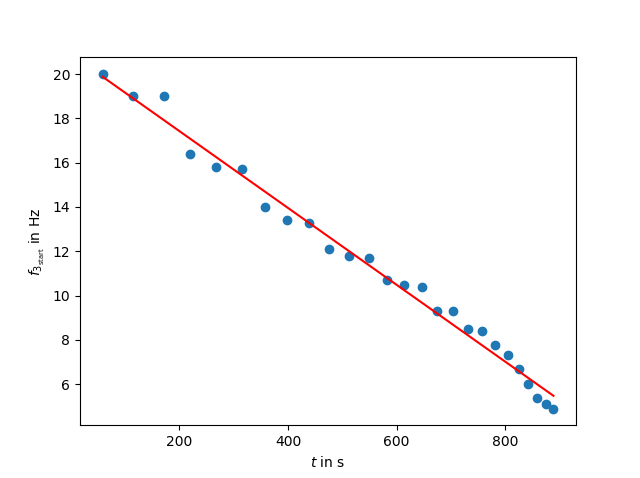
\includegraphics[scale=0.7]{6_3-Linear.png}
\end{figure}
Damit ist die Winkelgeschwindigkeit $\omega_3^i$ im jeweiligen Intervall $i$ gegeben durch 
\begin{align}
    \omega_3^i=2\pi\frac{f_{3_{start}}^i+f_{3_{end}}^i}{2}=\pi(f_{3_{start}}^i+f_{3_{end}}^i)
\end{align}
Der Fehler des Stroboskop wird abgeschätzt mit $u_{f_3} = 0.25$ Hz. Zwar liegt der Ablesefehler des Stroboskop $u_a = 0.005$ Hz, aber durch die verwendet Messmethode wäre dies eine zu optimistischer Fehler, da die Messperson immer nur ein kleines Zeitfenster hatte um ungefähr die richtige Frequenz am Stroboskop einzustellen. Mit dem Fehlerfortpflanzungsgesetz ergibt sich dann der Fehler $u_{\omega_3^i}$ mit
\begin{align}
    u_{\omega_3^i}=\sqrt{2}\pi u_{f_3}
\end{align}
Weierhin ist die Präzessionswinkelgeschwindigkeit $\omega_p^i$ mit dem Fehler $u_{\omega_p^i}$ für die jeweiligen Intervalle $i$ gegeben 
\begin{gather}
    \omega_p^i=\frac{2\pi}{T^i}\tab u_{\omega_p^i}=\frac{2\pi}{(T^i)^2}u_T
\end{gather}
wobei der Fehler der Stoppuhr mit dem Ablesefehler abgeschätzt wird $u_a=u_T=0.01$ s.\\
Das Produkt aus $\omega_3^i$ und $\omega_p^i$ wird abgekürzt mit $\omega_*^i$. Den Fehler $u_{\omega_*^i}$ des Produkts erhält aus dem Fehlerfortpflanzungsgesetz und ist gegeben durch
\begin{align}
    u_{\omega_\ast^i}=\sqrt{(w_3^i u_{w_p^i})^2+(w_p^i u_{w_3^i})^2}
\end{align}
\begin{center}
    \captionof{table}{Messreihe 1}
    \begin{tabular}{gccccccccccc}
        \rowcolor[rgb]{ .741,  .843,  .933}{} &      $\omega_3$ $[\frac{1}{s}]$ &  $u_{\omega_3}$ $[\frac{1}{s}]$ &    $\omega_p$ $[\frac{1}{s}]$ &     $u_{\omega_p}$ $[\frac{1}{s}]$ &     $\omega_*$ $[\frac{1}{s^2}]$&  $u_{\omega_*}$ $[\frac{1}{s^2}]$\\
        1  &  109.30 &  1.11 &  0.11 &  0.00002 &  12.31 &  0.13 \\
        2  &   91.29 &  1.11 &  0.13 &  0.00003 &  12.29 &  0.15 \\
        3  &   78.70 &  1.11 &  0.15 &  0.00004 &  12.00 &  0.17 \\
        4  &   69.93 &  1.11 &  0.17 &  0.00005 &  12.15 &  0.19 \\
        5  &   62.08 &  1.11 &  0.19 &  0.00006 &  12.10 &  0.22 \\
        6  &   55.79 &  1.11 &  0.22 &  0.00007 &  12.05 &  0.24 \\
        7  &   51.08 &  1.11 &  0.24 &  0.00009 &  12.09 &  0.26 \\
        8  &   47.38 &  1.11 &  0.25 &  0.00010 &  12.08 &  0.28 \\
        9  &   43.92 &  1.11 &  0.28 &  0.00012 &  12.22 &  0.31 \\
        10 &   40.21 &  1.11 &  0.30 &  0.00014 &  11.97 &  0.33 \\
    \end{tabular}\\
    \captionof{table}{Messreihe 2}
    \begin{tabular}{gccccccccccc}
        \rowcolor[rgb]{ .741,  .843,  .933}{} &      $\omega_3$ $[\frac{1}{s}]$ &  $u_{\omega_3}$ $[\frac{1}{s}]$ &    $\omega_p$ $[\frac{1}{s}]$ &     $u_{\omega_p}$ $[\frac{1}{s}]$ &     $\omega_*$ $[\frac{1}{s^2}]$&  $u_{\omega_*}$ $[\frac{1}{s^2}]$\\
        1 &  114.35 &  1.11 &  0.11 &  0.00002 &  12.29 &  0.12 \\     
        2 &   95.50 &  1.11 &  0.13 &  0.00003 &  12.16 &  0.14 \\     
        3 &   82.00 &  1.11 &  0.15 &  0.00003 &  12.08 &  0.16 \\     
        4 &   71.66 &  1.11 &  0.17 &  0.00005 &  12.06 &  0.19 \\     
        5 &   63.74 &  1.11 &  0.19 &  0.00006 &  12.09 &  0.21 \\
    \end{tabular}\\
    \newpage
    \captionof{table}{Messreihe 3}
    \begin{tabular}{gccccccccccc}
        \rowcolor[rgb]{ .741,  .843,  .933}{} &      $\omega_3$ $[\frac{1}{s}]$ &  $u_{\omega_3}$ $[\frac{1}{s}]$ &    $\omega_p$ $[\frac{1}{s}]$ &     $u_{\omega_p}$ $[\frac{1}{s}]$ &     $\omega_*$ $[\frac{1}{s^2}]$&  $u_{\omega_*}$ $[\frac{1}{s^2}]$\\
        1 &  109.01 &  1.11 &  0.11 &  0.00002 &  12.09 &  0.12 \\     
        2 &   91.42 &  1.11 &  0.13 &  0.00003 &  12.11 &  0.15 \\     
        3 &   78.85 &  1.11 &  0.15 &  0.00004 &  12.20 &  0.17 \\     
        4 &   69.43 &  1.11 &  0.17 &  0.00005 &  11.96 &  0.19 \\     
        5 &   61.89 &  1.11 &  0.20 &  0.00006 &  12.18 &  0.22 \\     
        6 &   55.64 &  1.11 &  0.22 &  0.00007 &  12.04 &  0.24 \\      
        7 &   50.71 &  1.11 &  0.24 &  0.00009 &  11.99 &  0.26 \\ 
    \end{tabular}
\end{center}
Bei der Messreihe 4 kann man deutlich erkennen, dass das Produkt $\omega_*$ weit von dem Wert der anderen Messreihen abweicht. Es wird vermutet, dass hier ein systematischer Fehler vorliegt, weswegen diese aus der weiteren Auswertung ausgeschlossen wird. 
\begin{center}
    \captionof{table}{Messreihe 4}
    \begin{tabular}{gccccccccccc}
        \rowcolor[rgb]{ .741,  .843,  .933}{} &      $\omega_3$ $[\frac{1}{s}]$ &  $u_{\omega_3}$ $[\frac{1}{s}]$ &    $\omega_p$ $[\frac{1}{s}]$ &     $u_{\omega_p}$ $[\frac{1}{s}]$ &     $\omega_*$ $[\frac{1}{s^2}]$&  $u_{\omega_*}$ $[\frac{1}{s^2}]$\\
        1 &  35.75 &  1.11 &  0.37 &  0.00022 &  13.15 &  0.41 \\      
        2 &  32.89 &  1.11 &  0.39 &  0.00024 &  12.82 &  0.43 \\      
        3 &  31.35 &  1.11 &  0.41 &  0.00026 &  12.76 &  0.45 \\      
        4 &  29.91 &  1.11 &  0.43 &  0.00030 &  12.99 &  0.48 \\
    \end{tabular}
\end{center}
Durch die Auswertung wird deutlich, dass $\omega_*$ um einen bestimmten Wert gestreut ist. 
\begin{figure}[ht]
    \centering
    \caption{$w_*$ Histogramm}
    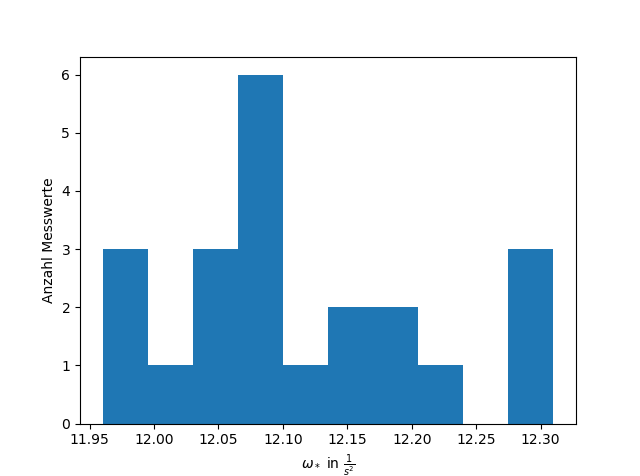
\includegraphics[scale=0.6]{6_3-Hist.png}
\end{figure}
Weswegen wir hier den Mittelwert über alle Messreihen bilden. Der Fehler der Mittelwertbildung wird mit dem Fehlerfortpflanzungsgesetz ermittelt und ist gegeben durch
\begin{align}
    u_{\overline{\omega_*}}=\frac{1}{N}\sqrt{\sum_{i=1}^{N} u_{\omega_*^i}^2}\tab N:\text{Anzahl der Intervalle}
\end{align}
Somit folgt das Ergebnis:
\begin{align*}
    \Rightarrow\boxed{\overline{w_*}=(12.11 \pm 0.04)~\frac{1}{s^2}}
\end{align*}
In Abb 4.5 lässt sich auch die Schwankung der Messwerte der einzelen Messreihen gut erkennen. Dabei ist anzumerken, dass für ähnliche Werte von $w_3$ der Unterschied von $w*$ zwischen den Messreihen stark schwankt, aber im Rahmen der Messgenauigkeit bleibt.\\ \\
Um das Trägheitsmoment $J_3$ zu berechnen wir Gleichung (2.13) aus Kapitel 2.5 umgeformt
\begin{align}
    \omega_p = \frac{mgl}{J_3\omega_3}~\Leftrightarrow~\omega_p\omega_3 = \omega_* = \frac{mgl}{J_3}~\Leftrightarrow~J_3 = \frac{mgl}{\omega_*}
\end{align}
Da die Massestückchen beide um einiges weniger wiegen als die gesamte Kugel mit Stab wird von einer neuen Berechnung des Schwerpunkts abgesehen. Dafür wird aber aufgrund der ähnlichen Masse der einzelnen Massestückchen Schwerpunkt in der Mitte der Massenstückchen angenommen. Die Erdbeschleunigung wird als fehlerfrei mit $g=9.81~\frac{m}{s^2}$ angenommen. \\
Der Fehler der Masse $m$ wird mit dem Ablesefehler $s_a=0.5~g$, welcher zugeleich auch als Restfehler $s_r$ angenommen wird, angeben als
\begin{align}
    u_m=\sqrt{s_a^2+s_r^2}=\sqrt{2}s_a=0.70710678~g
\end{align}
Weiterhin wird die Länge l bestimmt mit der Formel und den Werten $s_s=87.00~mm,~s_m=15.00~mm,~h_m=10.00~mm~d_k=100.00~mm~d_f=96.00~mm$
\begin{align}
    l = d_f - \left(\frac{d_k}{2}\right) + s_s - s_m - h_m=108.00~mm 
\end{align}
Die Längen wurden mit einem Messschieber vermessen, dessen Restfehler \\ $s_r=0.05~mm+1\cdot10^{-4}l$ im Praktikumsskript auf S. (F-5) zu finden ist. Der Ablesefehler liegt bei $s_a=0.05~mm$ und es wird die selbe Formel wie in (4.14) angewendet.
\begin{center}
    \begin{tabular}{ccccc}
        \rowcolor[rgb]{ .741,  .843,  .933}  $u_{s}~[mm]$ &  $u_{s_m}~[mm]$ &  $u_{h_m}~[mm]$ &  $u_{d_k}~[mm]$ &  $u_{d_f}~[mm]$\\
        0.07710830 & 0.07142128 & 0.07177917 & 0.07779562 & 0.078102496
    \end{tabular}
\end{center}
Womit der Fehler der Länge l mit dem Fehlerfortpflanzungsgesetz angeben werden kann
\begin{align}
    u_l=\sqrt{u_s^2+u_{s_m}^2+u_{h_m}^2+\left(\frac{u_{d_k}}{2}\right)^2+u_{d_f}^2}=0.16740370~mm
\end{align}
\begin{align*}
    \Rightarrow\boxed{m=(48.2\pm0.7)~g\tab l=(108,00\pm0.17)~mm}
\end{align*}
Daraus folgt für die Berechnung des Trägheitsmoments $J_3$ und dessen Fehler (über Fehler), wobei für $\omega_*$ der gebildete Mittelwert $\overline{\omega_*}$ verwendet wird. 
\begin{gather}
    J_3 = 4.21692287\cdot10^{-3}kgm^2 \\
    s_{J_3}=\sqrt{\left(\frac{gl}{\overline{\omega_*}}u_m\right)^2+\left(\frac{mg}{\overline{\omega_*}}u_l\right)^2+\left(\frac{mgl}{\overline{\omega_*}^2}u_{\overline{\omega_*}}\right)^2}=0.063255404~\cdot10^{-3}kgm^2
\end{gather}
\begin{align*}
    \Rightarrow\boxed{J_3=(4.21\pm0.06)\cdot10^{-3}kgm^2}
\end{align*}
Mit dem Trägheitsmoment $J_3$ wird nun mit Gleichung (4.4) das Trägheitsmoment $J_1$ bzgl. der 1. Hauptachse berechnet, wobei auch hier für $\omega_N$ der errechnete Mittelwert verwendet wird.
\begin{gather}
    \overline{\omega_N}=\frac{J_3-J_1}{J_1}~\Leftrightarrow~ J_1=\frac{J_3}{1+\overline{\omega_N}}=4.27889013\cdot 10^{-3}kgm^2\\
    u_{J_1}=\sqrt{\left(\frac{u_{J_3}}{1+\overline{\omega_N}}\right)^2+\left(\frac{J_3u_{\overline{\omega_N}}}{(1+\overline{\omega_N})^2}\right)^2}=0.069957618\cdot 10^{-3}kgm^2
\end{gather}
\begin{align*}
    \Rightarrow\boxed{J_1=(4.28\pm0.07)\cdot10^{-3}kgm^2}
\end{align*}
Prinzipell entspricht das Ergebnis unseren Erwartungen, da $J_3<J_1$ erfüllt wurde. Ist das Trägheitsmoment und seine Dimension bekannt kann man damit die Dichte das Körpers errechnen. In diesem Fall handelt es sich um eine Stahlkugel der Dichte $\rho = 7850~\frac{kg}{m^3}$ \footnote{\url{https://www.chemie.de/lexikon/Stahl.html#:~:text=Die%20Dichte%20von%20Stahl%20bzw,zu%201530%C2%B0C%20betragen.}}.\\
Für das Trägheitsmoment einer Kugel gilt folgender Zusammenhang:
\begin{align}
    J=\frac{8}{15}\rho\pi r^5 ~\Leftrightarrow~ \rho=\frac{15 J}{8\pi r^5}
\end{align}
Setzt man nun für $J$ das Trägheitsmoment $J_3$ ein und nimmt an, dass der Kreisel näherungsweise eine Kugel ist, erhält man für $\rho\approx8040~\frac{kg}{m^3}$ was in richtigen Größenordnung liegt und für die Richtigkeit der Ergebnisse spricht.
\newpage
\begin{figure}[ht]
    \centering
    \caption{$w_3$-$w_*$ Diagramm}
    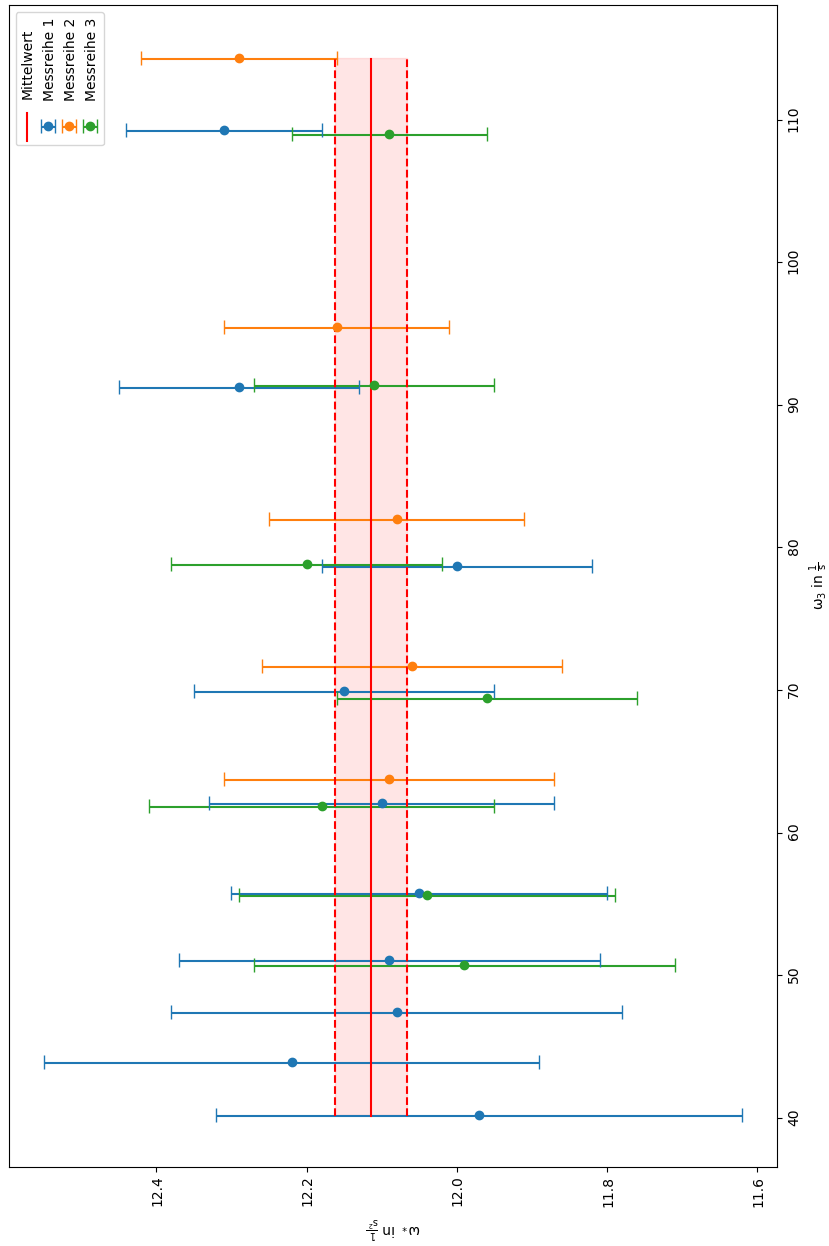
\includegraphics[scale=0.6]{6_3-Praezession.png}
\end{figure}
